% Previous horizontal figure preserved for review:
% % Figure 2(a): values from
% % vcomp/experiments/paper_evidence/current/fig_bg_loading/displayed_values.tsv.
% % WAF is total RocksDB SST bytes written divided by application logical input.
% \begin{tikzpicture}[
%     x=1cm,
%     y=1cm,
%     font=\normalsize,
%     axis/.style={draw=black!75, line width=0.45pt},
%     grid/.style={draw=black!12, line width=0.35pt},
%     oneKB/.style={draw=blue!75!black, fill=blue!65},
%     ninetyB/.style={draw=red!75!black, fill=red!65},
%     oneKBWaf/.style={draw=blue!85!black, dashed, line width=0.8pt},
%     ninetyBWaf/.style={draw=red!85!black, dashed, line width=0.8pt}
% ]
% \path[use as bounding box] (-0.30,-0.05) rectangle (6.05,4.80);
% \draw[axis] (0.75,0.95) -- (5.35,0.95);
% \draw[axis] (0.75,0.95) -- (0.75,4.15);
% 
% % Logarithmic y-axis from 0.5 h to 100 h.
% \foreach \y/\label in {0.950/0.5,1.369/1,2.759/10,4.150/100} {
%     \draw[grid] (0.75,\y) -- (5.35,\y);
%     \draw[axis] (0.70,\y) -- (0.75,\y);
%     \node[anchor=east, font=\normalsize] at (0.64,\y) {\label};
% }
% 
% % Right linear y-axis: standard input-normalized WAF from 10 to 23.
% \draw[axis] (5.35,0.95) -- (5.35,4.15);
% \foreach \y/\label in {0.950/10,1.935/14,2.919/18,3.904/22} {
%     \draw[axis] (5.35,\y) -- (5.40,\y);
%     \node[anchor=west, font=\normalsize] at (5.46,\y) {\label};
% }
% % Keep the secondary-axis title inside panel (a), away from panel (b)'s
% % vertical loading-time label.
% \node[anchor=south east, font=\Large] at (5.25,4.20) {WAF};
% 
% % x / DB size (TiB) / 1KB time (h) / 91B time (h)
% \foreach \x/\db/\vOne/\vNinety in {
%     1.30/0.5/0.623611111/2.733888889,
%     2.20/1/1.358055556/5.597500000,
%     3.10/2/2.834166667/11.235555556,
%     4.00/4/5.946111111/23.685833333,
%     4.90/8/13.251111111/46.226027778
% } {
%     \pgfmathsetmacro{\yOne}{0.95 + 3.20*ln(\vOne/0.5)/ln(200)}
%     \pgfmathsetmacro{\yNinety}{0.95 + 3.20*ln(\vNinety/0.5)/ln(200)}
%     \draw[oneKB] (\x-0.18,0.95) rectangle (\x,\yOne);
%     \draw[ninetyB] (\x,0.95) rectangle (\x+0.18,\yNinety);
%     \node[anchor=north, font=\normalsize] at (\x,0.89) {\db};
% }
% 
% % Standard WAF, using the same color as each loading-time series.
% % 1 KB: 12.35498, 14.00085, 16.054005, 18.5980125, 20.77557625.
% \draw[oneKBWaf]
%     (1.30,1.529687) -- (2.20,1.934825) -- (3.10,2.440217) --
%     (4.00,3.066434) -- (4.90,3.602450);
% \foreach \x/\y in {
%     1.30/1.529687,2.20/1.934825,3.10/2.440217,
%     4.00/3.066434,4.90/3.602450
% } {
%     \filldraw[draw=blue!85!black, fill=white, line width=0.65pt]
%         (\x,\y) circle (0.065);
% }
% 
% % 91 B: 13.48798, 15.2994, 17.47122, 20.1236325, 22.086965.
% \draw[ninetyBWaf]
%     (1.30,1.808580) -- (2.20,2.254468) -- (3.10,2.789070) --
%     (4.00,3.441971) -- (4.90,3.925253);
% \foreach \x/\y in {
%     1.30/1.808580,2.20/2.254468,3.10/2.789070,
%     4.00/3.441971,4.90/3.925253
% } {
%     \filldraw[draw=red!85!black, fill=white, line width=0.65pt]
%         (\x,\y) circle (0.065);
% }
% 
% \node[rotate=90, anchor=south, font=\Large] at (-0.02,2.55)
%     {Loading time (hour)};
% \node[anchor=north, font=\normalsize] at (3.05,0.43) {DB size (TiB)};
% \draw[oneKB] (1.02,4.34) rectangle (1.34,4.58);
% \node[anchor=west, font=\normalsize] at (1.44,4.46) {1KB};
% \draw[ninetyB] (2.72,4.34) rectangle (3.04,4.58);
% \node[anchor=west, font=\normalsize] at (3.14,4.46) {91B};
% \end{tikzpicture}

% Active vertical figure generated from the promoted TSV data.
% Figure 2(a): values from
% vcomp/experiments/paper_evidence/current/fig_bg_loading/displayed_values.tsv.
% WAF is total RocksDB SST bytes written divided by application logical input.
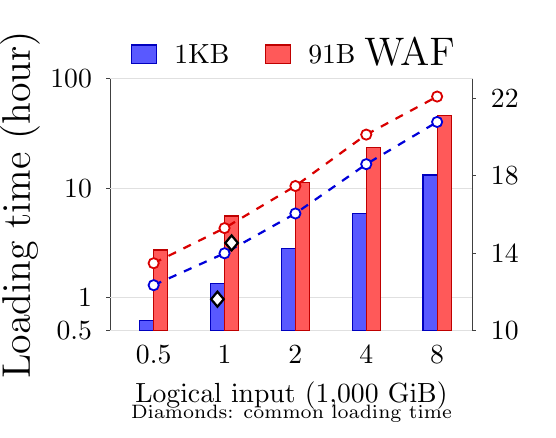
\begin{tikzpicture}[
    x=1cm,
    y=1cm,
    font=\normalsize,
    axis/.style={draw=black!75, line width=0.45pt},
    grid/.style={draw=black!12, line width=0.35pt},
    oneKB/.style={draw=blue!75!black, fill=blue!65},
    ninetyB/.style={draw=red!75!black, fill=red!65},
    oneKBWaf/.style={draw=blue!85!black, dashed, line width=0.8pt},
    ninetyBWaf/.style={draw=red!85!black, dashed, line width=0.8pt}
]
\path[use as bounding box] (-0.30,-0.05) rectangle (6.05,4.80);
\draw[axis] (0.75,0.95) -- (5.35,0.95);
\draw[axis] (0.75,0.95) -- (0.75,4.15);

% Logarithmic y-axis from 0.5 h to 100 h.
\foreach \y/\label in {0.950/0.5,1.369/1,2.759/10,4.150/100} {
    \draw[grid] (0.75,\y) -- (5.35,\y);
    \draw[axis] (0.70,\y) -- (0.75,\y);
    \node[anchor=east, font=\normalsize] at (0.64,\y) {\label};
}

% Right linear y-axis: standard input-normalized WAF from 10 to 23.
\draw[axis] (5.35,0.95) -- (5.35,4.15);
\foreach \y/\label in {0.950/10,1.935/14,2.919/18,3.904/22} {
    \draw[axis] (5.35,\y) -- (5.40,\y);
    \node[anchor=west, font=\normalsize] at (5.46,\y) {\label};
}
% Keep the secondary-axis title inside panel (a), away from panel (b)'s
% vertical loading-time label.
\node[anchor=south east, font=\Large] at (5.25,4.20) {WAF};

% x / Logical input (1,000 GiB) / 1KB time (h) / 91B time (h)
\foreach \x/\db/\vOne/\vNinety in {
    1.30/0.5/0.623611111/2.733888889,
    2.20/1/1.358055556/5.597500000,
    3.10/2/2.834166667/11.235555556,
    4.00/4/5.946111111/23.685833333,
    4.90/8/13.251111111/46.226027778
} {
    \pgfmathsetmacro{\yOne}{0.95 + 3.20*ln(\vOne/0.5)/ln(200)}
    \pgfmathsetmacro{\yNinety}{0.95 + 3.20*ln(\vNinety/0.5)/ln(200)}
    \draw[oneKB] (\x-0.18,0.95) rectangle (\x,\yOne);
    \draw[ninetyB] (\x,0.95) rectangle (\x+0.18,\yNinety);
    \node[anchor=north, font=\normalsize] at (\x,0.89) {\db};
}

% Standard WAF, using the same color as each loading-time series.
% 1 KB: 12.35498, 14.00085, 16.054005, 18.5980125, 20.77557625.
\draw[oneKBWaf]
    (1.30,1.529687) -- (2.20,1.934825) -- (3.10,2.440217) --
    (4.00,3.066434) -- (4.90,3.602450);
\foreach \x/\y in {
    1.30/1.529687,2.20/1.934825,3.10/2.440217,
    4.00/3.066434,4.90/3.602450
} {
    \filldraw[draw=blue!85!black, fill=white, line width=0.65pt]
        (\x,\y) circle (0.065);
}

% 91 B: 13.48798, 15.2994, 17.47122, 20.1236325, 22.086965.
\draw[ninetyBWaf]
    (1.30,1.808580) -- (2.20,2.254468) -- (3.10,2.789070) --
    (4.00,3.441971) -- (4.90,3.925253);
\foreach \x/\y in {
    1.30/1.808580,2.20/2.254468,3.10/2.789070,
    4.00/3.441971,4.90/3.925253
} {
    \filldraw[draw=red!85!black, fill=white, line width=0.65pt]
        (\x,\y) circle (0.065);
}

\node[rotate=90, anchor=south, font=\Large] at (-0.02,2.55)
    {Loading time (hour)};
\node[anchor=north, font=\normalsize] at (3.05,0.43) {Logical input (1,000 GiB)};
\draw[oneKB] (1.02,4.34) rectangle (1.34,4.58);
\node[anchor=west, font=\normalsize] at (1.44,4.46) {1KB};
\draw[ninetyB] (2.72,4.34) rectangle (3.04,4.58);
\node[anchor=west, font=\normalsize] at (3.14,4.46) {91B};
% Common release / 16-buffer 1,000-GiB measurements, unconnected diamonds.
\draw[draw=black,fill=white,line width=0.8pt] (2.1100,1.4469)--(2.1900,1.3519)--(2.1100,1.2569)--(2.0300,1.3519)--cycle;
\draw[draw=black,fill=white,line width=0.8pt] (2.2900,2.1612)--(2.3700,2.0662)--(2.2900,1.9712)--(2.2100,2.0662)--cycle;
\node[font=\scriptsize,anchor=north] at (3.05,0.13) {Diamonds: common loading time};
\end{tikzpicture}
